\chapter{Desenvolvimento}
\label{chap:desenvolvimento}

Neste capítulo serão apresentadas todas as etapas referentes ao desenvolvimento da ferramenta
WikiOlapBase (WOB), que permite a integração de dados abertos de forma colaborativa. Na seção
\ref{sec:requisitos} serão explicitados os requisitos levantados para a ferramenta. 
Posteriormente, na seção \ref{sec:arquitetura}, será mostrada a arquitetura proposta para o 
WOB. Finalmente, na seção \ref{sec:wob}, a ferramenta será apresentada, ainda nessa seção será 
apresentada uma análise comparativa entre o WOB e as ferramentas encontradas na literatura.

\section{Levantamento de Requisitos}
\label{sec:requisitos}

Na etapa de Levantamento de Requisitos foram definidas as funcionalidades e características 
do software proposto. Esse levantamento ocorreu a partir da revisão da literatura e através 
de uma reunião de \textit{brainstorming}, no dia 29 de abril de 2016, com três especialistas 
que possuem mais de oito anos de experiência na área de processamento e análise de dados. 
O resultado gerado foi a lista de requisitos, mostrada no Quadro \ref{quadro:requisitos}.

\begin{quadro}[!htb]
    \centering
    \caption{Requisitos do WOB}
    \label{quadro:requisitos}
    \begin{tabular}{|p{2cm}|p{13cm}|}
        \hline
        Identificador   &   Requisito \\
        \hline
        RF\_1    &  A ferramenta deve permitir a importação de dados, de forma a manter o significado dos dados originais \\   
        \hline
        RF\_2    &  A ferramenta deve ser capaz de converter diferentes formatos para o modelo de dados definido. \\        
        \hline
        RF\_3    &  A ferramenta deve permitir aos usuários o acesso aos dados presentes no banco de dados integrado da ferramenta. \\
        \hline
        RF\_4    &  A ferramenta deve permitir a definição de metadados que se relacionam com um determinado conjunto de dados. \\
        \hline
        RF\_5    &  A ferramenta deve ser capaz de estabelecer relacionamento entre conjunto de dados diferentes. \\
        \hline
        RF\_6    &  A ferramenta deve aceitar arquivos compactados \\
        \hline
        RF\_7    &  A ferramenta deve possibilitar a divisão dos conjuntos de dados em múltiplos arquivos para envio. \\        
        \hline
        RF\_8    &  A ferramenta deve disponibilizar uma interface para que outras aplicações acessem os dados presentes na base de dados integrada. \\
        \hline
        RNF\_1    &  A ferramenta deve ser capaz de armazenar dados em larga escala \\
        \hline
        RNF\_2    &  A ferramenta deve otimizar o tempo de consulta aos dados. \\ 
        \hline   
    \end{tabular}
    \fonte{O Autor}
\end{quadro}

A partir dos requisitos levantados foi possível escolher as tecnologias que permitiriam atender
tais requisitos, bem como propor uma arquitetura para a ferramenta. Na seção a seguir essas 
escolhas são expostas e justificadas.

\section{Arquitetura do WikiOlapBase}
\label{sec:arquitetura}

A arquitetura do WOB foi especificada de modo a definir: (1) a linguagem de 
programação utilizada, (2) o modelo de dados e os SGBDs utilizados, (3) a forma de acesso 
aos dados, e qualquer outra decisão de projeto. Essas decisões foram tomadas levando em 
consideração a revisão bibliográfica e os requisitos da ferramenta.

Para o desenvolvimento da ferramenta foi utilizado o padrão de arquitetura 
\textit{Model-View-Controller (MVC)}. Nesse padrão, o modelo de dados, a interface do 
usuário e lógica de controle são separados em três componentes: (1) o modelo, que 
representa a estrutura de dados e regras de negócio da aplicação, (2) a \textit{view}, 
que apresenta o modelo para o usuário e (3) o controlador, que interpreta a entrada do 
usuário e se comunica com o modelo para realizar as mudanças necessárias \cite{plekhanova2009evaluating}. 

Essa separação de conceitos, do inglês \textit{separation of concerns (SoC)}, permite o 
desenvolvimento e teste de cada componente de forma independente, o que facilita e agiliza o 
desenvolvimento. Isso também facilita a evolução das funcionalidades de aplicações web, o que 
justifica a escolha do padrão MVC para o desenvolvimento da ferramenta proposta 
\cite{gupta2012}. A Figura \ref{fig:mvc} mostra a interação entre os componentes no 
padrão MVC.

\begin{figure}[!htb]
    \centering
    \caption{Interação entre componentes do MVC}
    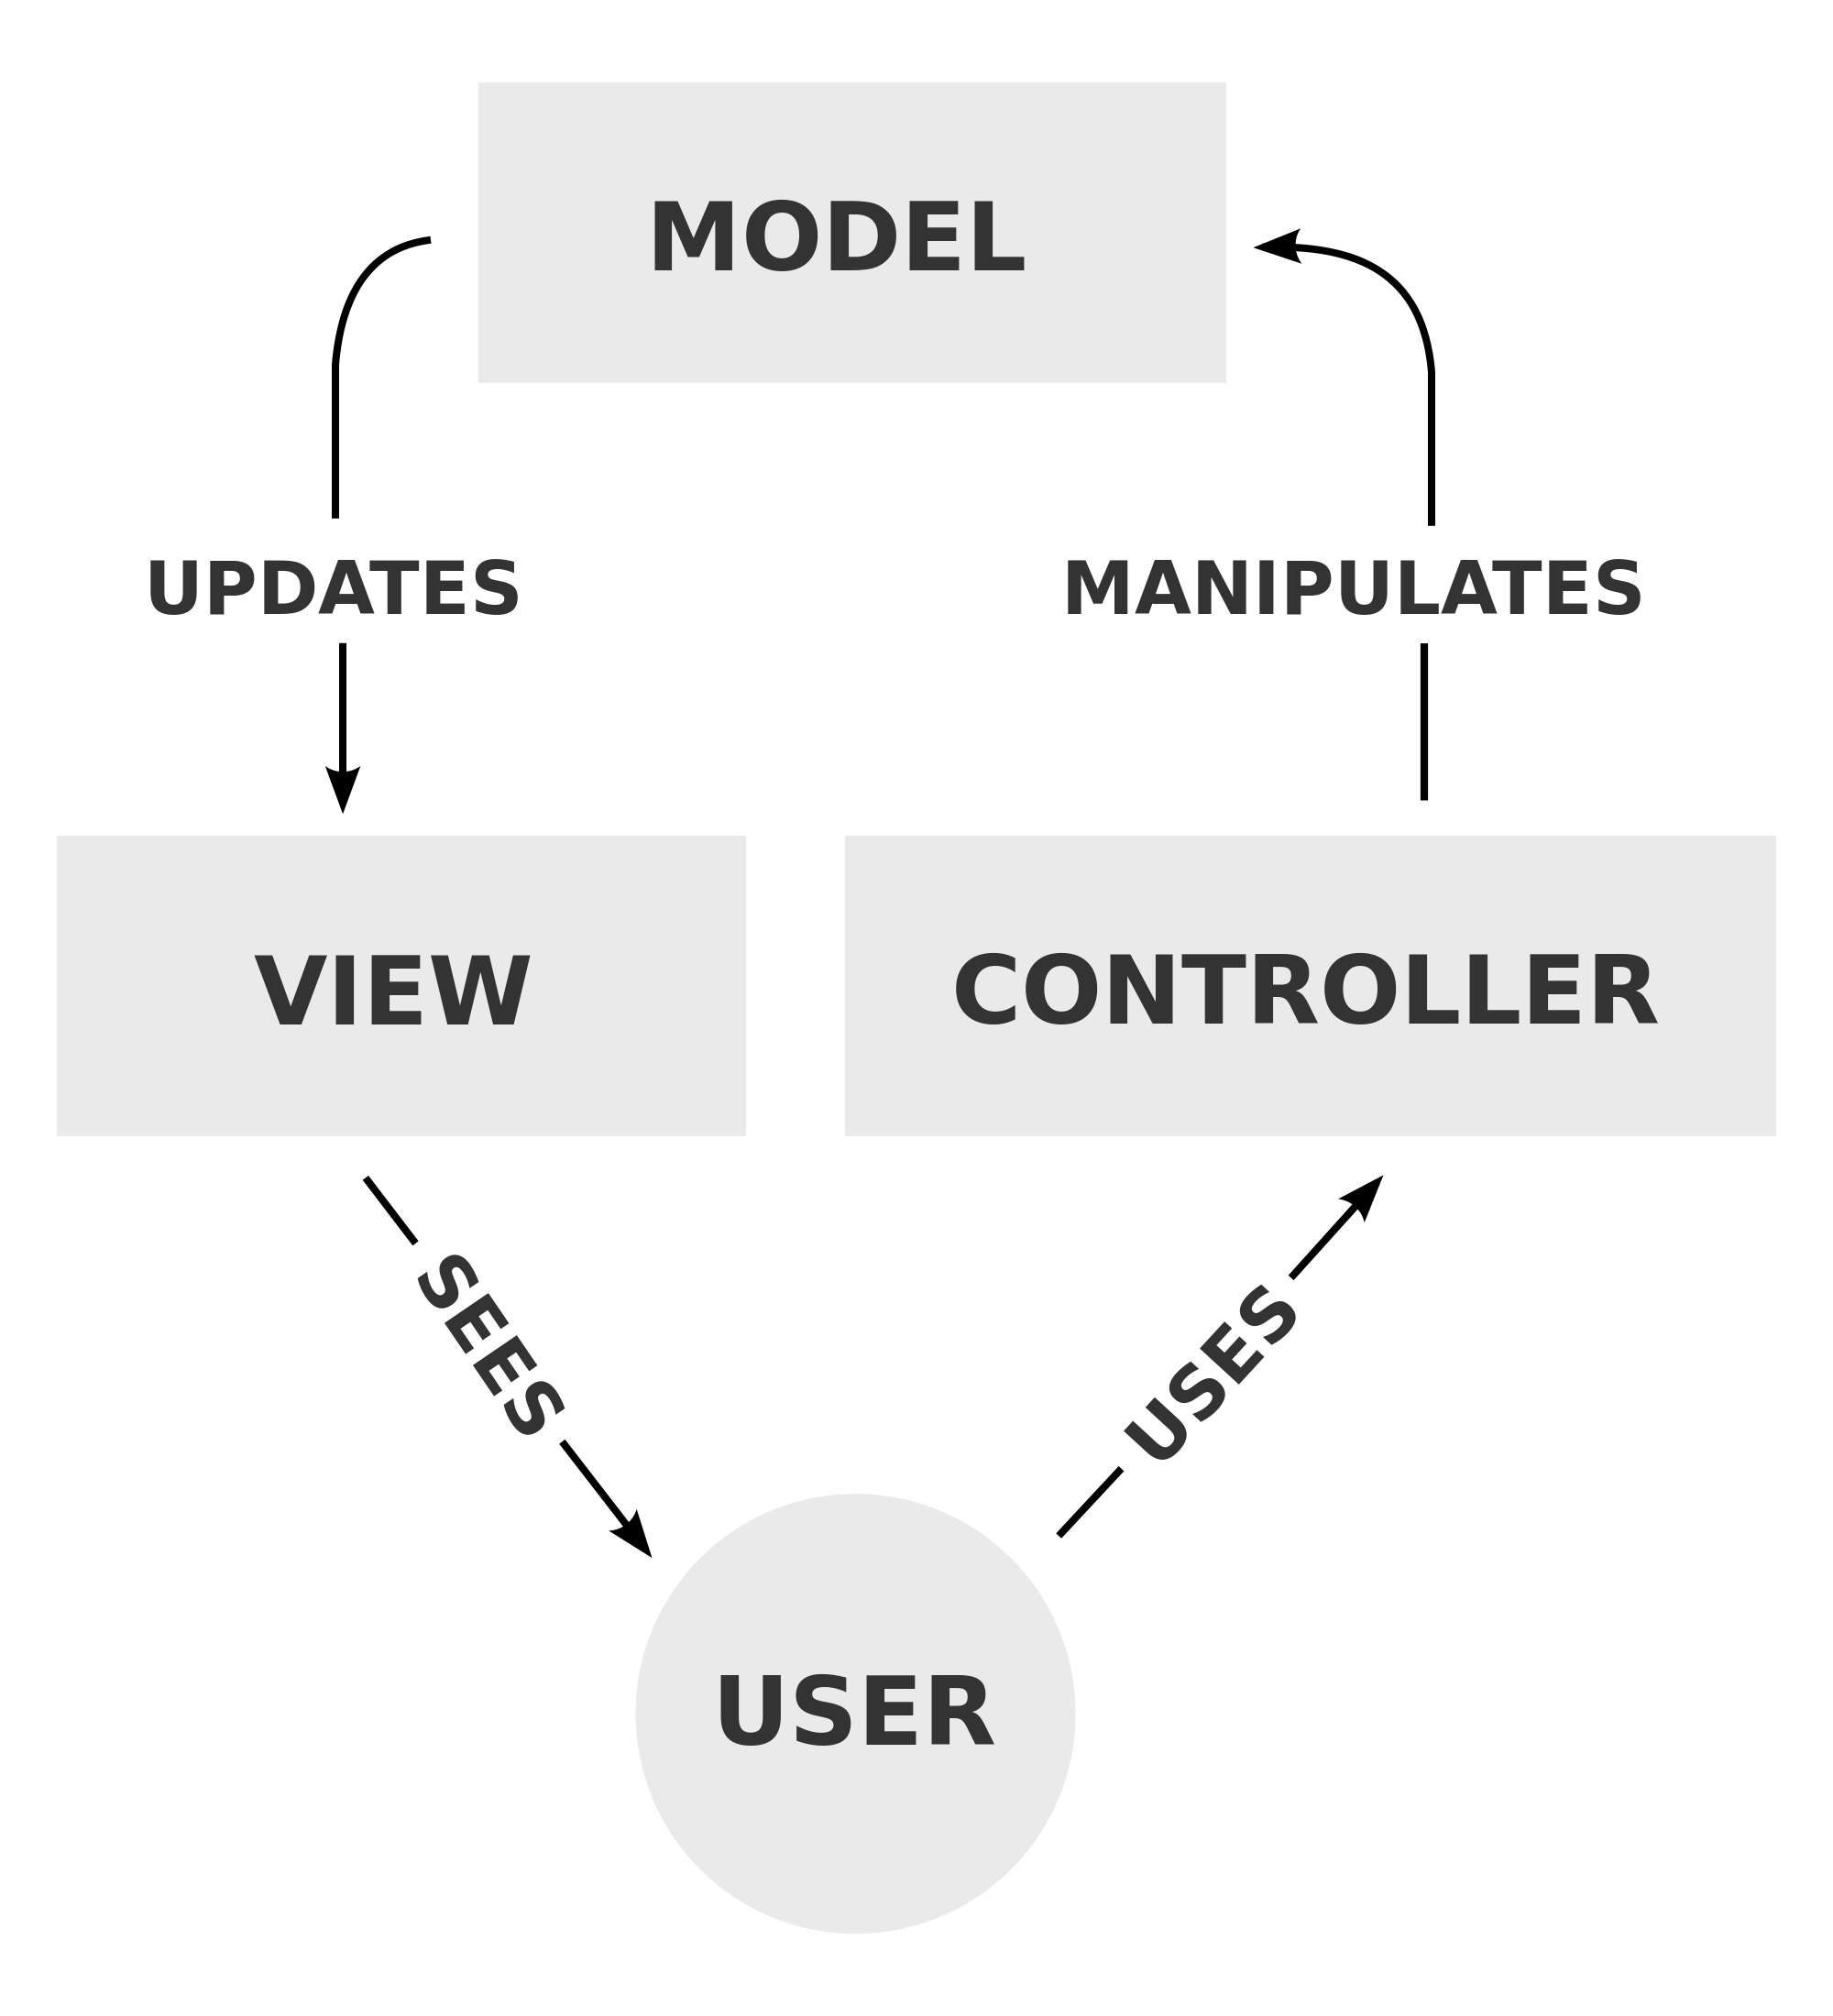
\includegraphics[width=0.4\textwidth]{./04-figuras/mvc}
    \fonte{\citeonline{wiki2016mvc}}
    \label{fig:mvc}
\end{figure}

Para a codificação da ferramenta foi utilizada a linguagem de programação Python, através do 
\textit{framework} Django. Python é uma linguagem de programação popular, que possui suporte 
para integração com outras linguagens e ferramentas, além de uma variedade de bibliotecas. 
Já o Django, é um \textit{framework} de código aberto que busca automatizar ao máximo o 
desenvolvimento, aderindo ao princípio \"não repita a si mesmo\", do inglês 
\textit{don’t repeat yourself (DRY)} \cite{plekhanova2009evaluating}. Também vale ressaltar 
que para a interface do usuário foram usadas as linguagens 
\textit{HyperText Markup Language} (HTML), \textit{Cascading Style Sheets (CSS)} e JavaScript.

A arquitetura aqui proposta busca funcionar como infraestrutura básica para ferramentas de
visualização de grandes volumes de dados que fazem uso de operações OLAP, e portanto, 
o modelo de dados escolhido deve viabilizar isso. Dessa forma, foi escolhido o modelo de 
família de colunas, pois ele otimiza esse tipo de operações, que tipicamente envolvem
consultas complexas em grandes porções de dados \cite{sorjonen2012olap}. 

Comparativamente, bancos de dados relacionais, orientados por linha, precisam manipular uma 
grande quantidade de itens para selecionar os dados necessários para responder a uma consulta, 
o que torna operações de leitura lentas, e portanto não indicadas quando se deixa realizar 
uma operação OLAP \cite{sorjonen2012olap}. Já bancos de dados orientados por coluna, acessam 
apenas os itens necessários para responder uma consulta, o que torna as operações de leitura
mais rápidas. Além disso, o modelo de família de colunas é mais escalável, o que no contexto
de grandes volumes de dados é uma característica desejada \cite{moniruzzaman2013nosql}.

Além dos conjuntos de dados que serão armazenados pela ferramenta, também foi necessário 
registrar os metadados referentes a esses conjuntos, de modo que seja possível 
caracterizá-los. Metadados são comumente definidos como dados sobre dados, no entanto, vão 
além dessa definição. Eles permitem ao usuário, ou um computador, procurar e gerenciar 
informações, definir as regras para uma estrutura de dados e integrar dados de diferentes 
fontes \cite{turner2002metadata}. Desse modo, para o armazenamento dos metadados, foi 
utilizado o modelo orientado a documentos. Esse modelo não possui 
estrutura definida, o que o torna uma boa escolha para armazenamento de metadados 
\cite{de2010nosql}.

O SGBD utilizado para implementar e gerenciar o modelo de família de colunas foi o 
Cassandra, já o modelo orientado a documentos foi implementado no MongoDB. 
Segundo o site db-engines.com (2016), esses dois SGBDs estão entre os dez mais utilizados, 
sendo os primeiros colocados em suas categorias. Isso demonstra a popularidade e aceitação 
da comunidade em relação a essas ferramentas, o que justifica suas escolhas. Devido as 
limitações dos bancos de dados NoSQL, já explorada anteriormente neste trabalho 
(na Seção \ref{sec:bigdata}), também foi utilizada a plataforma Spark para realizar uma 
interface com o Cassandra. A utilização do Spark permite a realização de operações mais 
complexas sobre os dados, além de tornar ainda mais rápida a leitura e escrita de dados 
sobre o Cassandra.

Finalmente, para o acesso aos dados, foi disponibilizado uma API REST, devido a sua 
simplicidade e adequação natural a web \cite{maleshkova2010}. A Figura \ref{fig:arquitetura} apresenta o 
diagrama da arquitetura implementada.  

\begin{figure}[!htb]
    \centering
    \caption{Arquitetura do WikiOlapBase}
    \includegraphics[width=0.6\textwidth]{./04-figuras/arquitetura}
    \fonte{O Autor}
    \label{fig:arquitetura}
\end{figure}

\section{WikiOlapBase}
\label{sec:wob}

A partir da arquitetura proposta na seção \ref{sec:arquitetura} e nos requisitos definidos
na seção \ref{sec:requisitos} a ferramenta WikiOlapBase foi implementada. Seu objetivo é
permitir a integração de dados abertos de forma colaborativa. O desenvolvimento foi iniciado
no dia 2 de junho de 2016 e a primeira versão funcional foi finalizada no dia 22 de setembro
de 2016, demorando, portanto, 3 meses e 20 dias.

A ferramenta proposta possui dois módulos: o primeiro é responsável por receber, caracterizar
e integrar os conjuntos de dados enviados pelos usuários, o segundo permite o acesso a esse 
repositório de dados integrados por meio de uma API REST. O primeiro módulo é composto por 
uma série de interfaces, nas quais os usuários preenchem os metadados referente a base de 
dados que está sendo enviada. O conjunto de dados é então processado e armazenado no 
Cassandra, já os metadados são armazenados no MongoDB. 

Para realizar o armazenamento no Cassandra, é utilizada uma API do Spark, o que torna esse 
processo mais rápido e eficaz \cite{kolaczkowski2014}. Já a API REST possui diversos métodos 
que podem ser acessados para realizar operações como: recuperação de dados, recuperação de 
metadados e cruzamento entre diferentes bases de dados. Para que o usuário possa recuperar 
e pré-processar os dados foi utilizada uma API do Spark que realiza essas operações de uma 
forma mais rápida \cite{kolaczkowski2014}. A seguir serão detalhados os principais passos 
do fluxo de execução da ferramenta.

O fluxo de execução principal do WOB é composto por quatro passos, para facilitar o 
aprendizado do usuário foi elaborada uma interface que explica esses passos, conforme
demonstrado nas Figuras \ref{fig:wob-ajuda}, \ref{fig:wob-ajuda2}, \ref{fig:wob-ajuda3} e
 \ref{fig:wob-ajuda4}.

\begin{figure}[!htb]
    \centering
    \caption{Interface de instruções do WOB - Passo 1}
    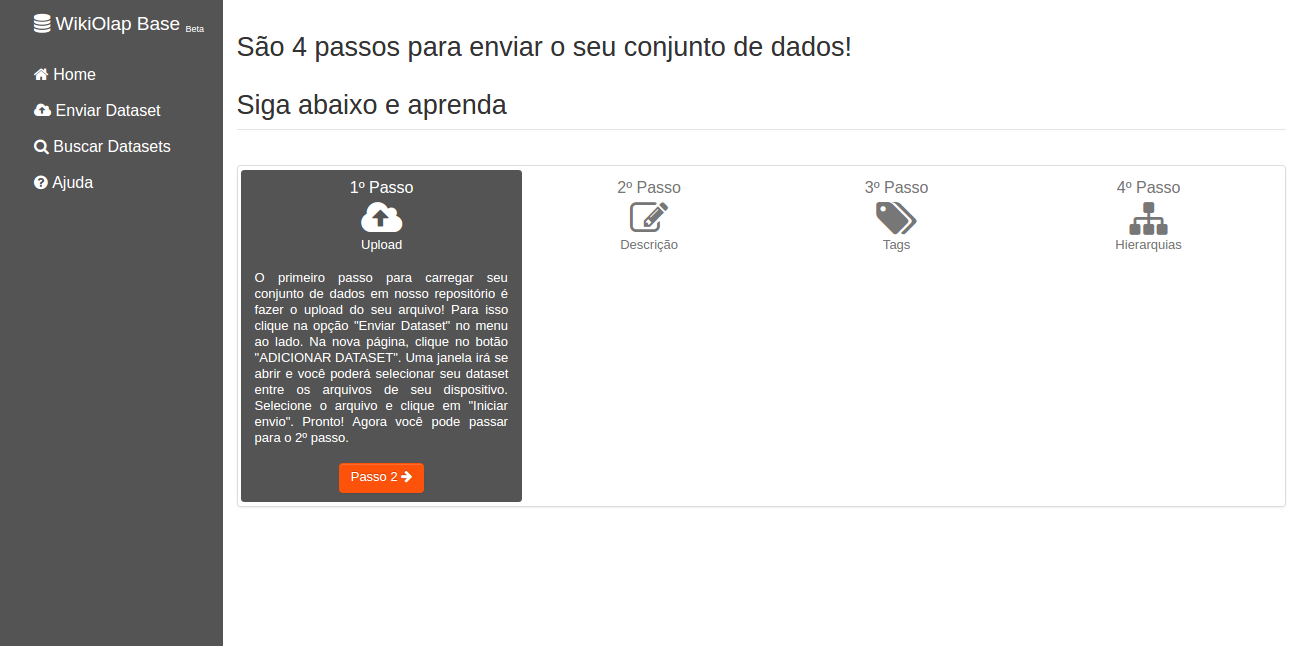
\includegraphics[width=0.87\textwidth]{./04-figuras/wob-ajuda}
    \fonte{O Autor}
    \label{fig:wob-ajuda}
\end{figure}

\begin{figure}[!htb]
    \centering
    \caption{Interface de instruções do WOB - Passo 2}
    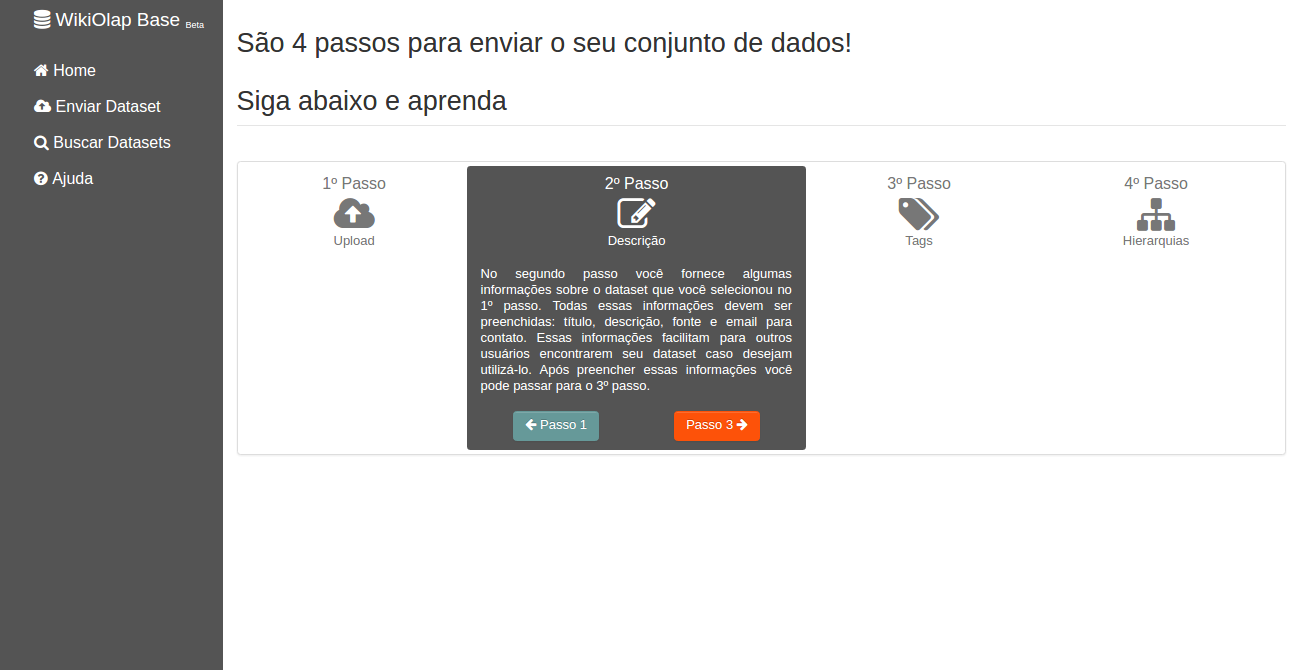
\includegraphics[width=0.87\textwidth]{./04-figuras/wob-ajuda2}
    \fonte{O Autor}
    \label{fig:wob-ajuda2}
\end{figure}

\begin{figure}[!htb]
    \centering
    \caption{Interface de instruções do WOB - Passo 3}
    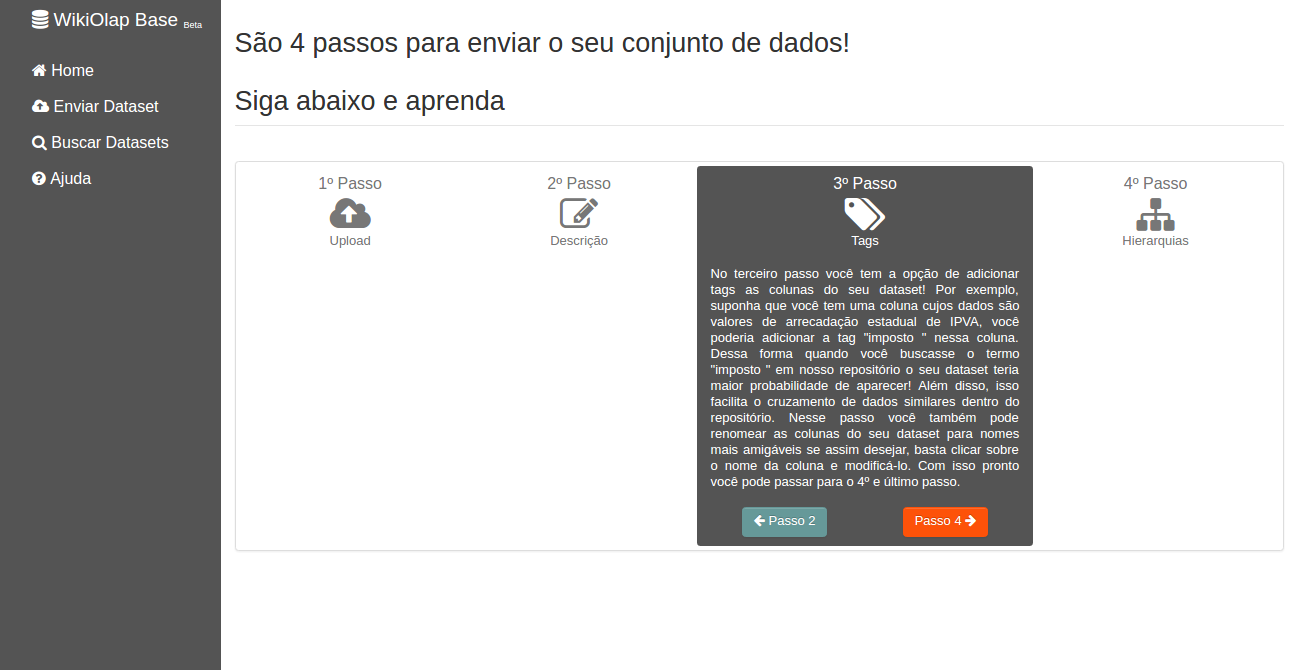
\includegraphics[width=1\textwidth]{./04-figuras/wob-ajuda3}
    \fonte{O Autor}
    \label{fig:wob-ajuda3}
\end{figure}

\begin{figure}[!htb]
    \centering
    \caption{Interface de instruções do WOB - Passo 4}
    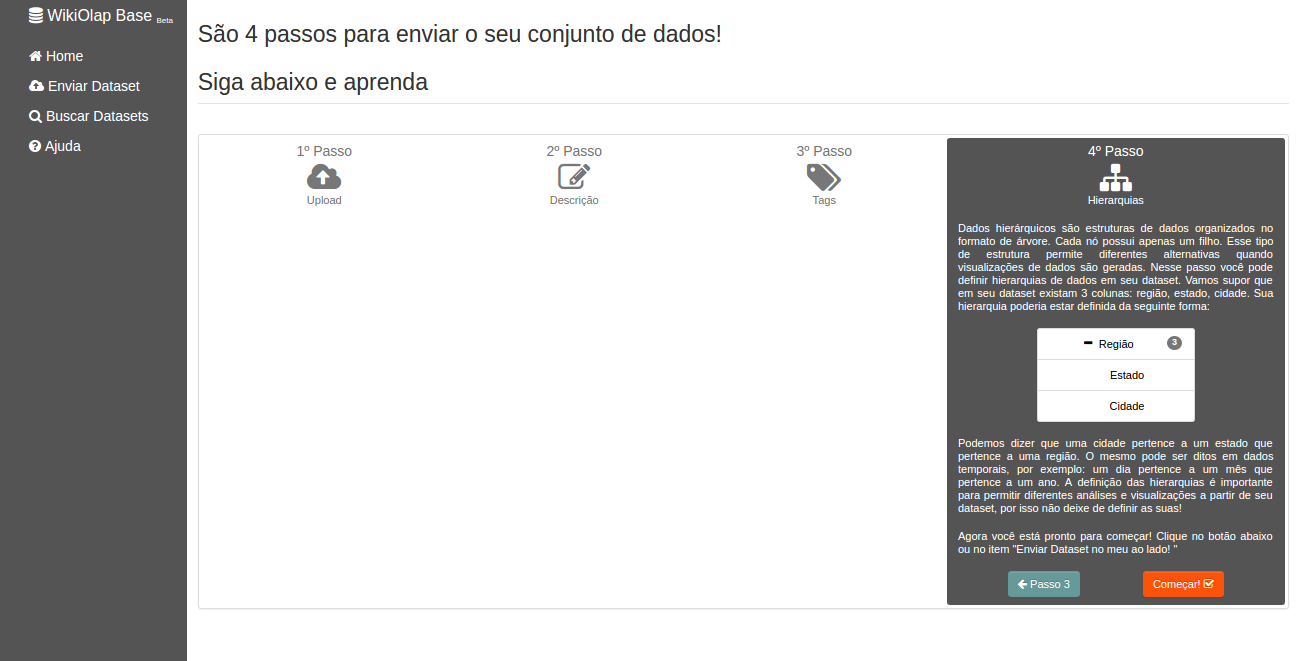
\includegraphics[width=1\textwidth]{./04-figuras/wob-ajuda4}
    \fonte{O Autor}
    \label{fig:wob-ajuda4}
\end{figure}

O primeiro passo de execução engloba a seleção e envio do conjunto de dados desejado, vale
ressaltar que nessa primeira versão só são aceitos arquivos no formato CSV, a Figura \ref{fig:wob-sendfile} 
mostra a interface elaborada para essas ações. A partir dos dados enviados o usuário deve 
preencher os metadados correspondentes, esse procedimento engloba os três passos de execução 
seguintes, embora seja sugerida uma sequência, o usuário pode realizar essa fase na ordem 
que desejar. 

\begin{figure}[!htb]
    \centering
    \caption{Interface para envio de arquivo do WOB}
    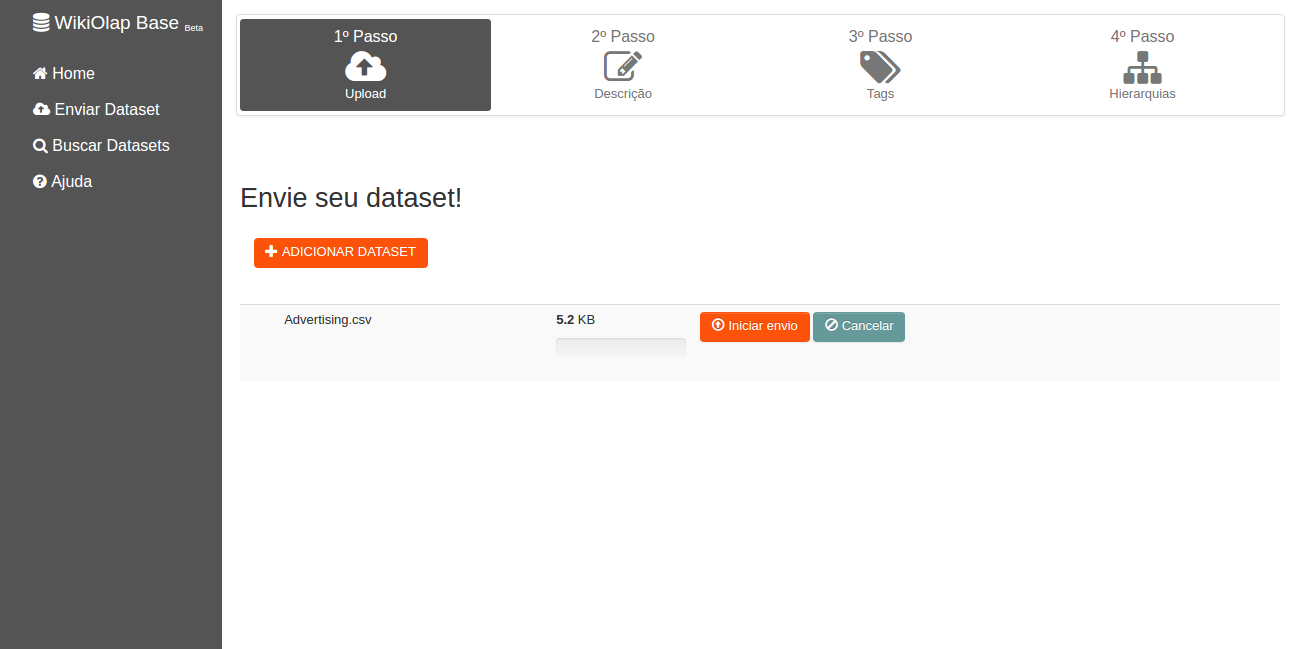
\includegraphics[width=1\textwidth]{./04-figuras/wob-sendfile}
    \fonte{O Autor}
    \label{fig:wob-sendfile}
\end{figure}

Seguindo a sequência sugerida, primeiro deve ser preenchido informações básicas do conjunto 
de dados, como fonte, título e descrição. Essas informações permitem a indexação dentro do 
repositório, possibilitando, posteriormente, que outros usuários possam buscar esses dados, 
a interface pode ser vista na Figura \ref{fig:wob-info}.

\begin{figure}[!htb]
    \centering
    \caption{Interface para preenchimento de informações básicas do WOB}
    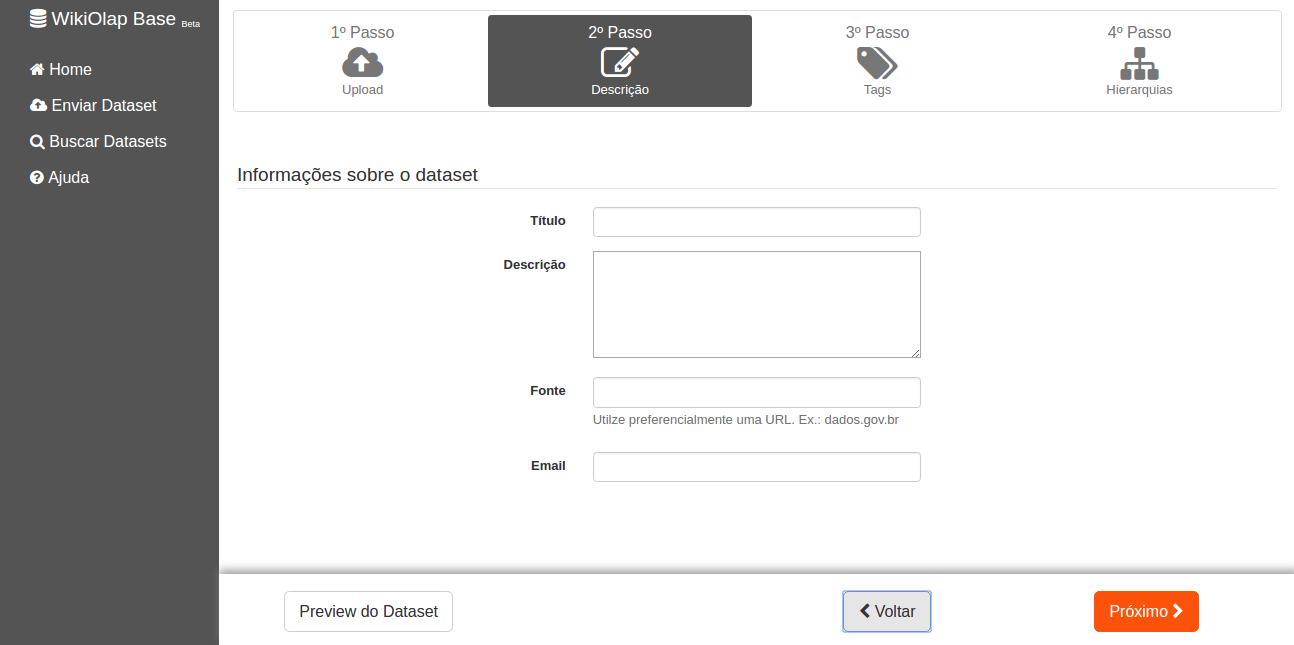
\includegraphics[width=1\textwidth]{./04-figuras/wob-info}
    \fonte{O Autor}
    \label{fig:wob-info}
\end{figure} \newpage


Logo depois, o usuário pode adicionar \textit{tags} às colunas do conjunto de dados. Isso, 
além de ajudar na indexação desses dados, também viabiliza o cruzamento entre conjuntos 
diferentes, pois permite a descoberta de conjuntos de dados que possuem atributos em comum. 
Nesse ponto o usuário também pode renomear as colunas, se assim o desejar, essa interface é 
mostrada na Figura \ref{fig:wob-tags}. 

\begin{figure}[!htb]
    \centering
    \caption{Interface para preenchimento de tags do WOB}
    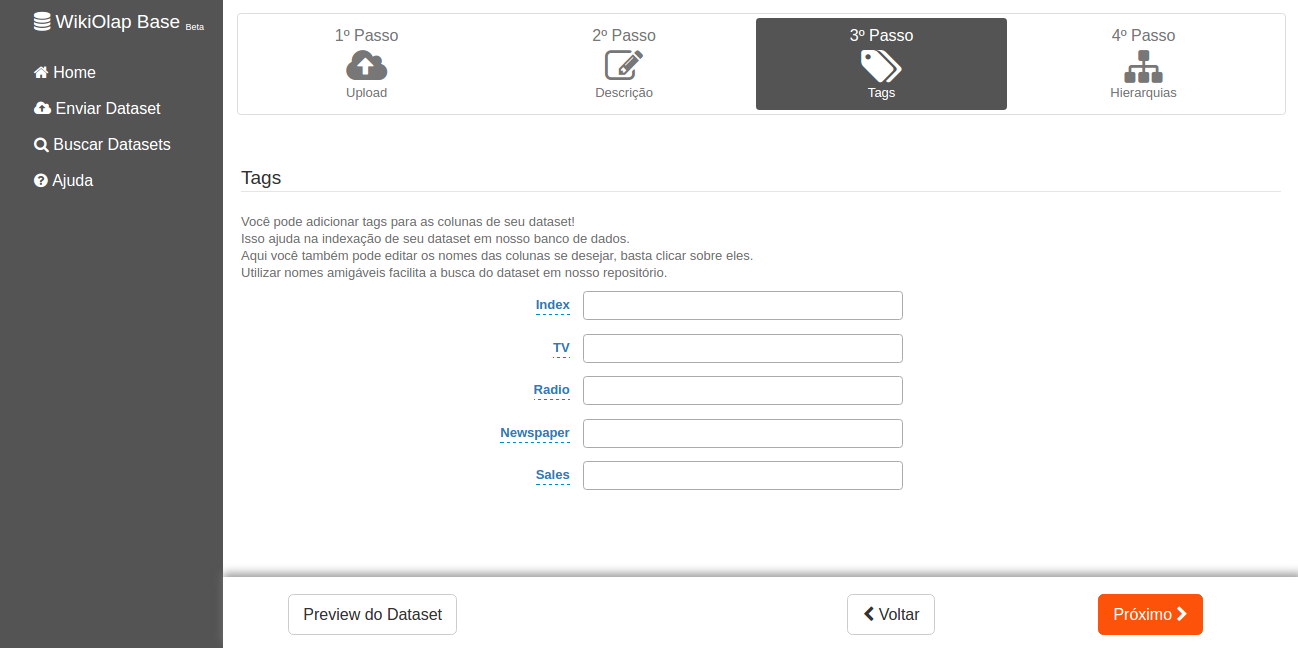
\includegraphics[width=1\textwidth]{./04-figuras/wob-tags}
    \fonte{O Autor}
    \label{fig:wob-tags}
\end{figure}

Por fim o usuário pode identificar hierarquias de dados dentro do conjunto enviado. Essa 
informação pode ser utilizada na geração de visualizações que utilizam operações OLAP como 
\textit{drill down} e \textit{drill up}, a interface pode ser vista na Figura \ref{fig:wob-hierarquia}. 
Além disso também é disponibilizado ao usuário um \textit{preview} de seu conjunto de dados, 
desse modo ele pode verificar se não ocorreu um erro ao enviar seu arquivo.

\begin{figure}[!htb]
    \centering
    \caption{Interface para indentificação de hierarquias do WOB}
    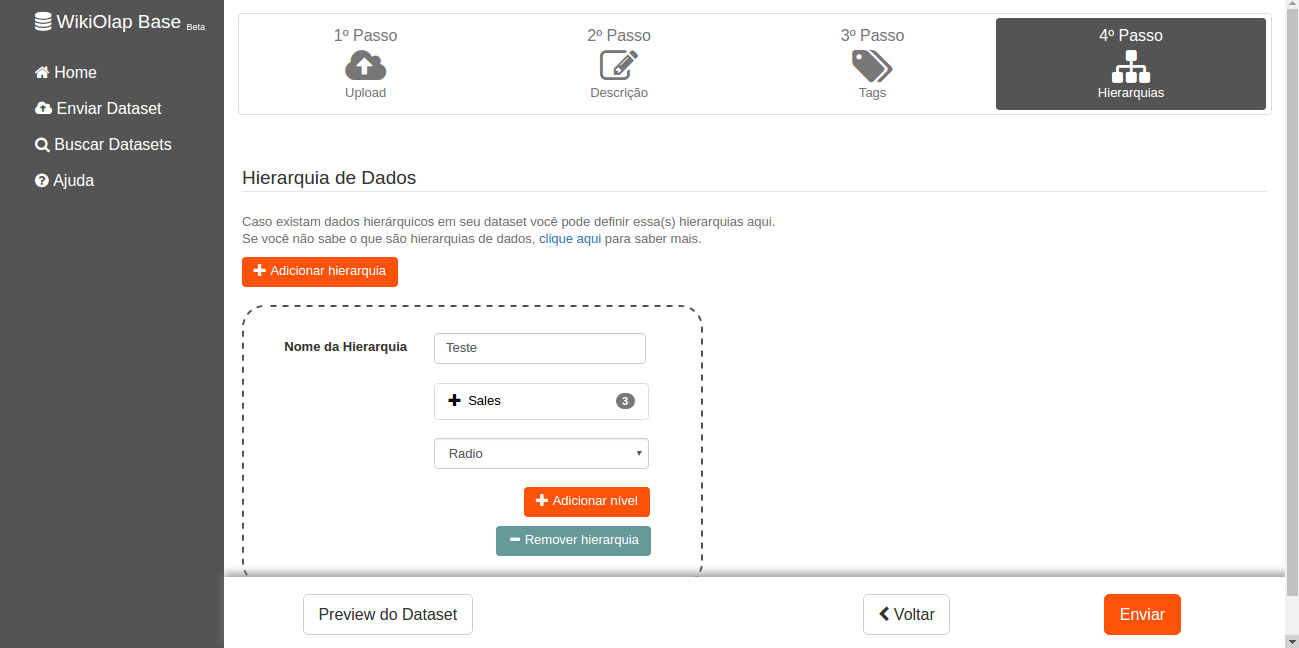
\includegraphics[width=1\textwidth]{./04-figuras/wob-hierarquia}
    \fonte{O Autor}
    \label{fig:wob-hierarquia}
\end{figure}

Essa sequência de ações, realizadas pelo usuário da ferramenta, viabiliza a integração entre
o conjunto de dados enviado por ele e os que já existem no repositório. Além disso, o 
preenchimento consciente dos metadados faz parte do aspecto colaborativo da ferramenta, 
já que isso possibilita a reutilização dos conjuntos enviados por qualquer usuário que 
assim o desejar.

Finalmente, para acessar o repositório do WikiOlapBase, e realizar operações em cima dos 
conjuntos de dados disponíveis, os usuários podem utilizar a API REST que foi desenvolvida, 
sua documentação\footnote{http://docs.wikiolapapi.apiary.io/} já se encontra disponível. 
Embora a ferramenta em si ainda não esteja disponível para o público em geral, o código 
fonte\footnote{https://github.com/pedromb/wikiolapbase} já é de domínio público.

Percebe-se que o WikiOlapBase possui algumas características que o diferenciam das outras ferramentas
mostradas no capítulo \ref{chap:trabRelac}. O Quadro \ref{quadro:comparativo2} mostra um 
comparativo entre as ferramentas e o WOB.

\begin{quadro}[!htb]
    \centering
    \caption{Comparação entre os sistemas encontrados na literatura e o WOB}
    \label{quadro:comparativo2}
    \begin{tabular}{|p{1.5cm}|p{1.5cm}|p{1.5cm}|p{1.5cm}|p{2cm}|p{2cm}|p{1.5cm}|p{1.5cm}|}
        \hline
Referên- cia & Modelo de Dados                & Forma de acesso aos dados            & Formato de importação dos dados                   & Importação de dados por usuários & Atualização colaborativa da base de dados & Disponibi- lização de metadados & Relacio- namento entre dados \\
        \hline
\citeonline{graves2013}          & Linked Data                    & Interface gráfica                    & Não especificado                                  & Não especificado                 & Não especificado                          & Sim      &    Não                     \\
        \hline          
\citeonline{hoxha2011open}         & Linked Data                    & Interface gráfica e consultas SPARQL & XML, CSV e texto             & Não                              & Não                                       & Sim      &    Não                      \\
        \hline
\citeonline{ding2010data}          & Linked Data                    & Webser- vice SPARQL                    & CSV                                               & Não                              & Não                                       & Sim      &    Não                     \\
        \hline
\citeonline{viegas2007}         & Tabela e texto não estruturado & Interface gráfica                    & Texto separado por tabulação.                     & Sim                              & Não                                       & Sim        &    Não                   \\
        \hline
\citeonline{tang2004}         & Relacio- nal                     & API REST                             & CSV, MDX e conexões SQL & Sim                              & Não                                       & Sim          &    Não                 \\
        \hline 
WikiOlap
Base         & Família de Colunas                     & API REST                             & CSV & Sim                              & Sim                                       & Sim                   &    Sim        \\
        \hline     
    \end{tabular}
    \fonte{O Autor}
\end{quadro} 

Pode-se observar que o WOB possui dois grandes diferenciais, o primeiro é o aspecto colaborativo,
já que todo gerenciamento da base de dados é feita pelos próprios usuários. O segundo diferencial
é a possibilidade de relacionar conjuntos de dados que estão disponíveis no repositório. 
Já um aspecto a ser melhorado pelo WOB é a disponibilidade de importação de dados em 
diferentes formatos, já que na versão inicial só está disponível o formato CSV.

Após o desenvolvimento da ferramenta foi realizada de uma avaliação de usabilidade,
com o objetivo de determinar se a ferramenta está adequada ao uso por parte do público alvo.
O capítulo seguinte mostra a metodologia utilizada e os resultados alcançados nessa avaliação.